\documentclass{article}
\usepackage{multicol}
\usepackage{tocloft}
%%%%Sửa đường dẫn tới subsection,section
\usepackage[colorlinks=true, linkcolor=blue
  ,hypertexnames=false% <- added
]{hyperref}
%%%%Sửa đường dẫn tới subsection,section
\usepackage{colortbl}
\usepackage[export]{adjustbox}
\usepackage{ragged2e}
\usepackage{verbatim}
\usepackage{marvosym}
\usepackage{pifont}
\usepackage{fontawesome}
\usepackage{fancyvrb}
\usepackage{comment}
\usepackage{accents}
\usepackage{algorithm} % Để sử dụng môi trường algorithm
\usepackage{algpseudocode} % Để sử dụng các câu lệnh trong pseudocode
\usepackage{diagbox}
\usepackage{helvet}
\usepackage{enumitem}
\usepackage{amssymb}
\usepackage{listings}
\usepackage{xcolor}
\definecolor{codegreen}{rgb}{0,0.6,0}
\definecolor{codegray}{rgb}{0.5,0.5,0.5}
\definecolor{codepurple}{rgb}{0.58,0,0.82}
\definecolor{backcolour}{rgb}{0.95,0.95,0.92}

\usepackage{listings}
\lstdefinestyle{mystyle}{
	backgroundcolor=\color{backcolour},   
	commentstyle=\color{codegreen},
	keywordstyle=\color{blue},
	numberstyle=\footnotesize\color{codegray},
	stringstyle=\color{codepurple},
	basicstyle=\ttfamily\small,
	breakatwhitespace=false,         
	breaklines=true,                 
	captionpos=b,                    
	keepspaces=true,                 
	%numbers=left,                    
	numbersep=10pt,                  
	showspaces=false,                
	showstringspaces=false,
	showtabs=false,                  
	tabsize=4,
	language=C++,
}
\lstset{style=mystyle}
\usepackage{tikz}
\usetikzlibrary{matrix}
\usetikzlibrary{positioning}
\usetikzlibrary{backgrounds}

\newcommand\numRowsK{3}
\newcommand\numColsK{3}
\newcommand{\K}[2]{% #1: row, #2: col
	\edef\Kcol##1##2##3{###2}%
	\edef\Krow##1##2##3{\noexpand\Kcol###1}%
	\Krow
	{1 0 1}
	{0 1 0}
	{1 0 1}%
}

\usepackage{pgfplots}
\pgfplotsset{width=8cm,compat=1.9}
\usetikzlibrary{calc}
\usepackage{tikz,tkz-tab}
\usetikzlibrary{arrows.meta}
\usepgfplotslibrary{fillbetween}
\usetikzlibrary{patterns}
\usepackage[utf8]{vietnam}
\renewcommand\thepart{\Alph{part}}
\renewcommand\thesection{\Roman{section}}
\renewcommand\thesubsection{\arabic{subsection}}
\usepackage{titlesec}
\titleformat*{\section}{\fontsize{20pt}{0pt}\selectfont \bfseries }
\usepackage{graphicx}
\usepackage{wrapfig}
\usepackage{float}
\usepackage{geometry}
\usepackage{fancyhdr}
\usepackage[framemethod=TikZ]{mdframed}
\usepackage{amsthm}
\geometry{a4paper,total={170mm,257mm},left=20mm,top=20mm,}
\usepackage{xcolor} 
\pagestyle{fancy} % header & footer
\fancyhf{} %xóa tất cả l c r head foot
\lhead{Computer Architecture - Nguyễn Xuân Huy Hoàng - 2311070} % đầu trái
\rfoot{Trang \thepage} %chân phải
\renewcommand{\headrulewidth}{1pt} % độ dày line
\renewcommand{\footrulewidth}{1pt}
\setcounter{secnumdepth}{4} % đếm số cho Heading 4 (1.1.1.1)
\setcounter{tocdepth}{4}
% HEADING 1
\titlespacing*{\section}{0pt}{0pt}{30pt} % a3 là d từ section tới dòng đầu tiên, a1 là d của sec so với lề trái
\titleformat*{\section}{\fontsize{16pt}{0pt}\selectfont \bfseries \centering} % a1 là size sec, a2 là d sec so với đầu trang 
%HEADING 2
\titlespacing*{\subsection}{0pt}{10pt}{10pt} 
\titleformat*{\subsection}{\fontsize{14pt}{0pt}\selectfont \bfseries}
% HEADING 3
\titlespacing*{\subsubsection}{0pt}{10pt}{10pt} 
\titleformat*{\subsubsection}{\fontsize{13pt}{0pt}\selectfont \bfseries \itshape  }
% HEADING 4
\titlespacing*{\paragraph}{0pt}{10pt}{0pt} 
\titleformat*{\paragraph}{\fontsize{11pt}{0pt}\selectfont \bfseries \itshape }
% Câu lệnh và các thư viện để chỉnh CAPTION
\renewcommand{\figurename}{\fontsize{13pt}{0pt}\selectfont \bfseries Hình}

\renewcommand{\thefigure}{\thesection.\arabic{figure}}
\usepackage{caption}
\captionsetup[Figure]{labelsep=space}

\renewcommand{\tablename}{\fontsize{13pt}{0pt}\selectfont \bfseries Table}
\renewcommand{\thetable}{\thesection.\arabic{table}}
\captionsetup[table]{labelsep=space}

\renewcommand{\theequation}{\thesection.\arabic{equation}}
%%%%%%%%%%%%%% Font chữ %%%%%%%%%%%%
\renewcommand{\familydefault}{\rmdefault}
%%%%%%%% Hyperref %%%%%%%%%%
\usepackage{hyperref}
\usepackage{footnotebackref}
\hypersetup{
    colorlinks=true,
    linkcolor=blue,
    filecolor=magenta,      
    urlcolor=cyan,
    pdftitle={Overleaf Example},
    pdfpagemode=FullScreen,
    }
\urlstyle{same}
%%%%%%%%%%%
\usepackage{mathtools}
\usepackage{bm}
\usepackage{esvect}
\title{\textbf{ĐẠI HỌC QUỐC GIA TP. HỒ CHÍ MINH}}
\author{\textbf{Trường Đại học Bách Khoa}}
\date{Khoa khoa học và kỹ thuật máy tính}


%%%%%%%%%%%%%%%%%%%%%%%%%%%%%%%%%%%%%%%%%%%%%%%
\newcounter{tongquat}[section] \setcounter{tongquat}{0}
\newenvironment{tongquat}[2][]{%
\refstepcounter{tongquat}%
\ifstrempty{#1}%
{\mdfsetup{%
frametitle={%
\tikz[baseline=(current bounding box.east),outer sep=0pt]
\node[anchor=east,rectangle,fill=blue!20]
{\strut Tổng quát};}}
}%
{\mdfsetup{%
frametitle={%
\tikz[baseline=(current bounding box.east),outer sep=0pt]
\node[anchor=east,rectangle,fill=blue!20]
{\strut Tổng quát};}}%
}%
\mdfsetup{innertopmargin=10pt,linecolor=blue!20,%
linewidth=2pt,topline=true,%
frametitleaboveskip=\dimexpr-\ht\strutbox\relax
}
\begin{mdframed}[]\relax%
\label{#2}}{\end{mdframed}}
%%%%%%%%%%%%%%%%%%%%%%%%%%%%%%%%%%%%%%%%%%%%%%%
%%%%%%%%%%%%%%%%%%%%%%%%%%%%%%%%%%%%%%%%%%%%%%%
\newcounter{chinhtac}[section] \setcounter{chinhtac}{0}
\newenvironment{chichtac}[2][]{%
\refstepcounter{chichtac}%
\ifstrempty{#1}%
{\mdfsetup{%
frametitle={%
\tikz[baseline=(current bounding box.east),outer sep=0pt]
\node[anchor=east,rectangle,fill=blue!20]
{\strut Chính tắc};}}
}%
{\mdfsetup{%
frametitle={%
\tikz[baseline=(current bounding box.east),outer sep=0pt]
\node[anchor=east,rectangle,fill=blue!20]
{\strut Chính tắc};}}%
}%
\mdfsetup{innertopmargin=10pt,linecolor=blue!20,%
linewidth=2pt,topline=true,%
frametitleaboveskip=\dimexpr-\ht\strutbox\relax
}
\begin{mdframed}[]\relax%
\label{#2}}{\end{mdframed}}
%%%%%%%%%%%%%%%%%%%%%%%%%%%%%%%%%%%%%%%%%%%%%%%
%%%%%%%%%%%%%%%%%%%%%%%%%%%%%%%%%%%%%%%%%%%%%%%
\newcounter{chuan}[section] \setcounter{chuan}{0}
\newenvironment{chuan}[2][]{%
\refstepcounter{chuan}%
\ifstrempty{#1}%
{\mdfsetup{%
frametitle={%
\tikz[baseline=(current bounding box.east),outer sep=0pt]
\node[anchor=east,rectangle,fill=blue!20]
{\strut Dạng chuẩn};}}
}%
{\mdfsetup{%
frametitle={%
\tikz[baseline=(current bounding box.east),outer sep=0pt]
\node[anchor=east,rectangle,fill=blue!20]
{\strut Dạng chuẩn};}}%
}%
\mdfsetup{innertopmargin=10pt,linecolor=blue!20,%
linewidth=2pt,topline=true,%
frametitleaboveskip=\dimexpr-\ht\strutbox\relax
}
\begin{mdframed}[]\relax%
\label{#2}}{\end{mdframed}}
%%%%%%%%%%%%%%%%%%%%%%%%%%%%%%%%%%%%%%%%%%%%%%%

\begin{document}

\begin{titlepage}
    \begin{tikzpicture}[overlay, remember picture]
\draw[line width=3pt]
    ($ (current page.north west) + (2.0cm,-2.0cm)$)
    rectangle
    ($ (current page.south east) + (-2.0cm,2.5cm)$);
\draw[line width=2pt]
    ($ (current page.north west) + (2.2 cm,-2.2cm)$)
     rectangle
    ($ (current page.south east) + (-2.2cm,2.7cm)$);

\end{tikzpicture}
\begin{center}
\vspace{1pt} {\large {BỘ GIÁO DỤC VÀ ĐÀO TẠO}} \\
\textbf{\fontsize{14pt}{0pt}\selectfont  ĐẠI HỌC QUỐC GIA THÀNH PHỐ HỒ CHÍ MINH }\\
\textbf{\fontsize{14pt}{0pt}\selectfont  TRƯỜNG ĐẠI HỌC BÁCH KHOA }\\
\rule{0.5\textwidth}{1pt}

\begin{figure}[h]
    \centering
    
\includegraphics[scale=0.45]{01_logobachkhoa.png}
\end{figure}
\vspace{1pt}
\fontsize{18pt}{0pt}\selectfont BÁO CÁO \\
\vspace{2pt}
\textbf{\fontsize{20pt}{0pt}\selectfont BỘ MÔN KIẾN TRÚC MÁY TÍNH }\\
\vspace{0.5cm}
\underline
{\fontsize{16pt}{1pt}\selectfont \textbf{CONVOLUTION OPERATION}}
\end{center}
\vspace{3.5cm}
\begin{center}
\vspace{0.5cm}
    \begin{tabular}{|w{l}{2cm}p{5.75cm}|}
    \hline
        \textbf{MSSV:} & 2311070 \\
        \hline
        \textbf{Họ và tên:} & Nguyễn Xuân Huy Hoàng \\
        \hline
        \textbf{Group:} & TN01 \\
        \hline
	\end{tabular}
\end{center}
\begin{center}
    \vspace{0.5cm}
    \textbf {
    \underline{Giảng viên hướng dẫn:} Nguyễn Thiên Ân}
\end{center}
\begin{center}
    \large \textbf{TP. Hồ Chí Minh, 2024}
\end{center}
\end{titlepage}

\newpage
\begin{center}
	\fontsize{18pt}{1pt} \selectfont \textbf{TÓM TẮT}
\end{center}
\begin{flushleft}
	\large
	\justifying
	\hspace{0.4cm} Tích chập (convolution) là một phép toán quan trọng trong lĩnh vực xử lý ảnh và trí tuệ nhân tạo, đặc biệt trong các mạng nơ-ron tích chập (CNN). Phép toán này cho phép máy tính học được các đặc trưng quan trọng của hình ảnh như cạnh, kết cấu, và hoa văn, từ đó hỗ trợ các ứng dụng nhận diện và phân tích hình ảnh. Trong các hệ thống phần cứng như MIPS, việc hiện thực hóa phép toán tích chập đòi hỏi những kỹ thuật tối ưu hóa để đảm bảo hiệu suất tính toán.
\end{flushleft}
\begin{flushleft}
	\large
	\justifying
	\hspace{0.4cm} Trong báo cáo này, tôi sẽ trình bày cách thực hiện phép toán tích chập trên kiến trúc tập lệnh MIPS, tập trung vào cài đặt thuật toán và tối ưu mã. Cụ thể, báo cáo sẽ mô tả cách thao tác với dữ liệu, thực hiện các phép toán ma trận và lưu trữ kết quả, cũng như các thách thức và giải pháp trong quá trình triển khai. Kết quả cho thấy việc thực hiện phép toán tích chập trên MIPS là khả thi và có thể đạt hiệu suất tốt khi sử dụng các kỹ thuật tối ưu phù hợp.
\end{flushleft}
\thispagestyle{empty}
\addtocontents{toc}{\protect\thispagestyle{empty}}
\clearpage



\thispagestyle{empty}
\addtocontents{toc}{\protect\thispagestyle{empty}}
\tableofcontents
\thispagestyle{empty}
\clearpage
\large


\newpage
\phantomsection
\clearpage
\section*{Giới thiệu}
\addcontentsline{toc}{section}{\protect\numberline{}Giới thiệu}
\setcounter{section}{1}\setlength{\baselineskip}{15pt}
   % đếm số cho section2, nếu không là hiện 0.1, 0.1.1
\setcounter{subsection}{0}
\setcounter{subsubsection}{0}
\large
\pagenumbering{arabic} % đánh số thứ tự 1,2,3,4,.....

\subsection{Giới thiệu về tích chập (Convolution Operation)}
\large
\hspace{0.4cm} Tích chập là một phép toán cơ bản trong học máy, đặc biệt là trong mạng nơ-ron tích chập (CNN). Phép toán này được áp dụng rộng rãi trong các hệ thống học sâu, đặc biệt trong các bài toán liên quan đến xử lý hình ảnh và video.\medskip

Tích chập liên quan đến việc di chuyển một bộ lọc (hay kernel) qua ma trận đầu vào, chẳng hạn như hình ảnh, và tính toán phép nhân điểm giữa bộ lọc và vùng cục bộ của ma trận đầu vào. Mỗi phép toán tích chập tạo ra một giá trị trong ma trận đầu ra, giúp tái tạo lại các đặc trưng của ảnh như cạnh, đường nét, hoặc hình dạng.\medskip

Quá trình này có thể được lặp lại nhiều lần để tạo ra các đặc trưng phức tạp hơn trong các lớp sâu của mạng nơ-ron. Điều này giúp mạng học được các đặc điểm không gian và cấu trúc từ dữ liệu, mà không cần phải xác định thủ công các đặc trưng như trong các phương pháp truyền thống.\medskip

\begin{center}
	\begin{tikzpicture}
		% ------- style -------
		\tikzset{%
			parenthesized/.style={%
				left delimiter  = (,
				right delimiter = ),
			},
			node distance = 10mu,
		}
		
		% ------- equation -------
		\matrix[matrix of math nodes, parenthesized] (I) {
			1 & 1 & 1 & 1 & 0 & 0 & 1 \\
			0 & 0 & 1 & 1 & 1 & 0 & 0 \\
			0 & 0 & 0 & 1 & 1 & 1 & 0 \\
			0 & 0 & 0 & 1 & 1 & 0 & 0 \\
			0 & 0 & 1 & 1 & 0 & 0 & 0 \\
			3 & 1 & 1 & 0 & 0 & 0 & 0 \\
			0 & 1 & 0 & 0 & 0 & 0 & 1 \\
		};
		
		\node (*) [right = of I] {${}*{}$};
		
		\newcommand\Kmatrix{}
		\foreach \row in {1, ..., 3} {
			\gdef \sep {}
			\foreach \col in {1, ..., 3} {%
				\xdef \Kmatrix {\unexpanded\expandafter{\Kmatrix}\unexpanded\expandafter{\sep}\noexpand \K{\row}{\col}}
				\gdef \sep { \& }
			}
			\xdef \Kmatrix {\unexpanded\expandafter{\Kmatrix}\noexpand\\}
		}
		\matrix[matrix of math nodes, parenthesized, ampersand replacement=\&] (K) [right = of *] {
			\Kmatrix
		};
		
		\node (=) [right = of K] {${}={}$};
		
		\matrix[matrix of math nodes, parenthesized] (I*K) [right = of {=}] {
			2 & 4 & 3 & 4 & 2 \\
			1 & 2 & 4 & 3 & 3 \\
			1 & 2 & 3 & 4 & 1 \\
			4 & 3 & 3 & 1 & 1 \\
			2 & 3 & 1 & 1 & 1 \\
		};
		
		% ------- highlighting -------
		\newcommand\rowResult{1}
		\newcommand\colResult{4}
		
		\begin{scope}[on background layer]
			\newcommand{\padding}{2pt}
			\coordinate (Is-nw) at ([xshift=-\padding, yshift=+\padding] I-\rowResult-\colResult.north west);
			\coordinate (Is-se) at ([xshift=+\padding, yshift=-\padding] I-\the\numexpr\rowResult+\numRowsK-1\relax-\the\numexpr\colResult+\numColsK-1\relax.south east);
			\coordinate (Is-sw) at (Is-nw |- Is-se);
			\coordinate (Is-ne) at (Is-se |- Is-nw);
			
			\filldraw[red,   fill opacity=.1] (Is-nw) rectangle (Is-se);
			\filldraw[green, fill opacity=.1] (I*K-\rowResult-\colResult.north west) rectangle (I*K-\rowResult-\colResult.south east);
			
			\draw[blue, dotted] 
			(Is-nw) -- (K.north west)
			(Is-se) -- (K.south east)
			(Is-sw) -- (K.south west)
			(Is-ne) -- (K.north east)
			;
			\draw[green, dotted] 
			(I*K-\rowResult-\colResult.north west) -- (K.north west)
			(I*K-\rowResult-\colResult.south east) -- (K.south east)
			(I*K-\rowResult-\colResult.south west) -- (K.south west)
			(I*K-\rowResult-\colResult.north east) -- (K.north east)
			;
			
			\draw[blue,  fill=blue!10!white] (K.north west) rectangle (K.south east);
			
			\foreach \row [evaluate=\row as \rowI using int(\row+\rowResult-1)] in {1, ..., \numRowsK} {%
				\foreach \col [evaluate=\col as \colI using int(\col+\colResult-1)] in {1, ..., \numColsK} {%
					\node[text=blue] at (I-\rowI-\colI.south east) [xshift=-.3em] {\tiny$\times \K{\row}{\col}$};
				}
			}
		\end{scope}
		
		% ------- labels -------
		\tikzset{node distance=0em}
		\node[below=of I] (I-label) {$Image$};
		\node at (K |- I-label)     {$Kernel$};
		\node at (I*K |- I-label)   {$Out = Image * Kernel$};
	\end{tikzpicture}%
\end{center}

\subsection{Tầm quan trọng của tích chập trong xử lý ảnh}
\large
\hspace{0.4cm} Tích chập là một trong những phép toán nền tảng trong các mô hình học sâu, đặc biệt là trong các mạng nơ-ron tích chập (CNN). Nhờ vào việc áp dụng các bộ lọc qua các vùng ảnh, mạng nơ-ron có thể phát hiện và học các đặc trưng quan trọng như đường biên, kết cấu và hình mẫu trong dữ liệu hình ảnh. Điều này đặc biệt quan trọng trong các ứng dụng như nhận diện hình ảnh, phân loại ảnh và phân tích video, nơi mà khả năng phát hiện các đặc trưng trong ảnh đóng vai trò quyết định đến hiệu quả của mô hình.

\subsection{Mục tiêu của báo cáo}
\large
\hspace{0.4cm} Mục tiêu của bài báo cáo này là phân tích và mô tả chi tiết mã nguồn về phép toán tích chập trong học sâu. Bài báo cáo sẽ cung cấp giải thích cụ thể về cách thức hoạt động của tích chập, từ việc di chuyển bộ lọc qua ảnh đầu vào đến việc tính toán các giá trị trong bản đồ đặc trưng. Bài báo cáo cũng sẽ làm rõ tầm quan trọng của tích chập trong việc phát hiện các đặc trưng trong hình ảnh, và từ đó, giúp hiểu sâu hơn về vai trò của tích chập trong các ứng dụng học sâu hiện đại. 
\newpage
\section*{Phép toán Tích chập}
\addcontentsline{toc}{section}{\protect\numberline{}Phép toán Tích chập}
\setcounter{section}{1}\setlength{\baselineskip}{15pt}
% đếm số cho section2, nếu không là hiện 0.1, 0.1.1
\setcounter{subsection}{0}
\setcounter{subsubsection}{0}
\large
\subsection{Một số khái niệm liên quan}
\begin{itemize}[label=$\square$]
	\item \textbf{Bước nhảy (Stride):} Xác định khoảng cách di chuyển của bộ lọc trên ma trận đầu vào. Bước nhảy lớn sẽ làm giảm kích thước đầu ra và ngược lại.
	\item \textbf{Đệm (Padding):} Giúp giữ nguyên kích thước của đầu vào khi áp dụng tích chập. Bằng cách thêm các phần tử 0 xung quanh đầu vào, đệm cho phép áp dụng phép tích chập mà không làm giảm kích thước ma trận đầu ra.
	\item \textbf{Bộ lọc (Filter/Kernel):} Xác định cách trích xuất đặc trưng. Các bộ lọc khác nhau sẽ phát hiện các đặc trưng khác nhau trong dữ liệu (ví dụ: cạnh, góc, họa tiết).
\end{itemize}
\subsection{Nguyên lý của phép toán tích chập}
\hspace{0.4cm} Phép toán tích chập giữa một ma trận đầu vào và một bộ lọc (kernel) được thực hiện theo các bước sau:

\begin{enumerate}
	\item \textbf{Đặt Bộ Lọc:} Đặt bộ lọc (kernel) lên một phần của ma trận đầu vào. Bộ lọc là một ma trận nhỏ (ví dụ: 3x3 hoặc 5x5) có các giá trị số, và những giá trị này sẽ ảnh hưởng đến cách trích xuất đặc trưng từ dữ liệu đầu vào.
	\item \textbf{Tính Giá Trị Tích Chập:}
	\begin{itemize}
		\item Tại vị trí hiện tại, tính tích chập bằng cách nhân từng phần tử của bộ lọc với phần tử tương ứng của đầu vào, rồi cộng tất cả các giá trị nhân đó lại.
		\item Kết quả là một giá trị duy nhất biểu diễn đặc trưng tại vị trí đó trong ma trận đầu vào.
	\end{itemize}
	\item \textbf{Dời Bộ Lọc:} Dời bộ lọc theo một bước di chuyển (stride) nhất định và lặp lại quá trình nhân và cộng trên toàn bộ ma trận đầu vào cho đến khi bộ lọc quét hết tất cả các vùng trong ma trận.
	\item \textbf{Tạo Ma Trận Đầu Ra:} Giá trị tại mỗi lần tính toán sẽ là một phần tử trong ma trận đầu ra, tạo thành bản đồ đặc trưng (feature map) – kết quả của phép tích chập.
\end{enumerate}

\begin{flushleft}
	\fontsize{14pt}{1pt} \selectfont \textbf{Công thức tính}
\end{flushleft}

Giả sử:

\begin{itemize}
	\item Ma trận đầu vào $image$ $I$, kích thước $N \times N$.
	\item Bộ lọc $kernel$ $K$, kích thước $M \times M$.
	\item Ma trận đầu ra $out$ $O$.
\end{itemize}

Công thức cho giá trị $O(x, y)$ tại vị trí $(x,y)$ của ma trận đầu ra là:
\begin{equation*}
	O(x, y) = \sum_{i=0}^{N-1} \sum_{j=0}^{N-1} I(x+i, y+j) \times K(i, j)
\end{equation*}

\subsection{Các ứng dụng điển hình của tích chập}
\begin{itemize}
	\item[$\square$] \textbf{Xử lý ảnh:} Tích chập dùng để làm mờ, tăng độ nét, phát hiện cạnh, và các tác vụ liên quan khác trong xử lý ảnh.
	\item[$\square$] \textbf{Mạng nơ-ron tích chập (CNN):} Tích chập giúp phát hiện các đặc trưng như cạnh, họa tiết, hoặc hình dạng trong ảnh để nhận diện và phân loại.
	\item[$\square$] \textbf{Xử lý tín hiệu:} Trong xử lý âm thanh và tín hiệu, tích chập giúp lọc và phân tích các đặc trưng tần số.
\end{itemize}

\pagebreak
\section*{Phân tích và cài đặt mã}
\addcontentsline{toc}{section}{\protect\numberline{}Phân tích và cài đặt mã}
\setcounter{section}{1}\setlength{\baselineskip}{15pt}
% đếm số cho section2, nếu không là hiện 0.1, 0.1.1
\setcounter{subsection}{0}
\setcounter{subsubsection}{0}
\large
\subsection{Sơ lược về mã nguồn}
\hspace{0.4cm} Đoạn mã gồm ba phần chính:

\begin{enumerate}
	\item \textbf{Xử lý đầu vào}: Phần đầu tiên xử lý chuỗi \texttt{input} từ file \texttt{input\_matrix.txt}. Phần này bao gồm việc đọc từng dòng để trích xuất các tham số như kích thước của ma trận, giá trị \texttt{padding}, và các giá trị cho cả ma trận ảnh (\texttt{image matrix}) và ma trận nhân (\texttt{kernel matrix}).
	
	\item \textbf{Padding ma trận và tích chập}: Sau khi xử lý xong phần đầu vào, mã sẽ tiến hành áp dụng \texttt{padding} cho ma trận ảnh như đã chỉ định. Sau đó, phép tích chập được thực hiện trên ma trận ảnh đã được padding bằng cách sử dụng ma trận \texttt{kernel}, cho ra một ma trận đầu ra (\texttt{output matrix}) là kết quả của phép tích chập.
	
	\item \textbf{Tạo đầu ra}: Cuối cùng, ma trận đầu ra sẽ được chuyển đổi thành chuỗi để có thể ghi vào file \texttt{output\_matrix.txt}. Chuỗi này được định dạng và lưu vào file, hoàn tất quá trình xử lý.
\end{enumerate}

\subsection{Xử lý đầu vào}
\begin{itemize}
	\item [$\square$] Xử lý dòng đầu tiên.
\end{itemize}
\begin{enumerate}
	\item \textbf{Mở file và lưu chuỗi đầu vào:} Đọc dữ liệu từ file \texttt{\textcolor{blue}{input\_matrix.txt}} vào một chuỗi.
	\item \textbf{Xử lý từng ký tự:} Bỏ qua khoảng trắng và dấu chấm, nếu là số thì lưu vào mảng.
	\item \textbf{Lưu các giá tri:} \textit{N, M, p, s} lần lượt cho \textit{size} của \textit{image, kernel, padding, stride}.
\end{enumerate}
\begin{algorithm}
	\caption{Pseudocode: \textit{\textbf{Mở file và xử lý dòng thứ nhất trong chuỗi đầu vào của input}}}
	\begin{algorithmic}[1]
		\State Open file \texttt{"input\_matrix.txt"}
		\State Save input string
		
		\Comment{Read and process the first line}
		\State \texttt{byte} $\gets$ first byte of (input string)
		\State \texttt{SoHangCot} $\gets$ is the address of the array that contains length elements
		\For{$i \gets 0$; $i \neq \texttt{endline character}$; $i \gets i + 1$}
		\If{\texttt{byte} = ' '}
		\State \texttt{byte} $\gets$ next(\texttt{byte}) \Comment{Skip the space character}
		\EndIf
		\If{\texttt{isNumber(byte)} = 1}
		\State \texttt{SoHangCot[i]} $\gets$ \texttt{isNumber(byte)}
		\State \texttt{byte} $\gets$ next(\texttt{byte})
		\EndIf
		\If{\texttt{byte} = '.'} \Comment{Skip the dot and the next adjacent character}
		\State \texttt{byte} $\gets$ next(\texttt{byte})
		\State \texttt{byte} $\gets$ next(\texttt{byte})
		\EndIf
		\EndFor
		\State $N \gets \texttt{SoHangCot[0]}$ The size of the image matrix
		\State $M \gets \texttt{SoHangCot[1]}$ The size of the kernel matrix
		\State $p \gets \texttt{SoHangCot[2]}$ The value of padding
		\State $s \gets \texttt{SoHangCot[3]}$ The value of stride
	\end{algorithmic}
\end{algorithm}
\pagebreak
\begin{itemize}
	\item [$\square$] Xử lý dòng thứ hai.
\end{itemize}
\begin{enumerate}
	\item \textbf{Khởi tạo địa chỉ cho mảng \texttt{image}: }Xác định \texttt{\textcolor{black}{image}} là địa chỉ của mảng lưu trữ các giá trị từ dòng đầu vào. 
	\item \textbf{Xử lý từng ký tự:} 
	\begin{itemize}
		\item \textbf{Bỏ qua khoảng trắng}: Nếu gặp.
		\item \textbf{Gán số nguyên}: Nếu ký tự là một số, lưu nó vào \texttt{image[i]}, rồi chuyển sang ký tự tiếp theo.
		\item \textbf{Xử lý chữ số thập phân}: Nếu ký tự là dấu chấm (\texttt{.}), bỏ qua dấu chấm và lấy tiếp chữ số liền sau, rồi nhân số đã lưu trong \texttt{image[i]} với 10 và cộng thêm chữ số mới.
	\end{itemize}
	\item \textbf{Lặp lại} cho đến khi kết thúc dòng, lưu tất cả các giá trị vào \texttt{image}.
\end{enumerate}
\begin{algorithm}
	\caption{Pseudocode: Xử lý dòng thứ hai trong chuỗi đầu vào của input}
	\begin{algorithmic}[1]
		\State \texttt{image} $\gets$ địa chỉ của mảng \texttt{image}
		\For{$i \gets 0$; $i \neq \texttt{endline character}$; $i \gets i + 1$}
		\If{\texttt{byte} = ' '}
		\State \texttt{byte} $\gets$ next(\texttt{byte})
		\EndIf
		\If{\texttt{isNumber(byte)}}
		\State \texttt{image[i]} $\gets$ \texttt{isNumber(byte)}
		\State \texttt{byte} $\gets$ next(\texttt{byte})
		\EndIf
		\If{\texttt{byte} = '.'}
		\State \texttt{byte} $\gets$ next(\texttt{byte})
		\State \texttt{image[i]} $\gets$ (\texttt{image[i]} * 10 + \texttt{isNumber(byte)}) * \texttt{signBIT}
		\EndIf
		\EndFor
	\end{algorithmic}
\end{algorithm}
\begin{itemize}
	\item [$\square$] Xử lý dòng thứ ba.
\end{itemize}
\begin{enumerate}
	\item \textbf{Khởi tạo địa chỉ cho mảng \texttt{kernel}: }Xác định \texttt{\textcolor{black}{kernel}} là địa chỉ của mảng lưu trữ các giá trị từ dòng đầu vào. 
	\item Cách xử lý tương tự với dòng thứ hai.
	\item Cách xử lý tương tự với dòng thứ hai.
\end{enumerate}
\begin{algorithm}
	\caption{Pseudocode: Xử lý dòng thứ ba trong chuỗi đầu vào của input}
	\begin{algorithmic}[1]
		\State \texttt{kernel} $\gets$ is the address of \texttt{kernel} matrix
		\For{$i \gets 0$; $i < \texttt{end of string}$; $i \gets i + 1$}
		\If{\texttt{bytes} = ' '}
		\State \texttt{bytes} $\gets$ next(\texttt{bytes})
		\EndIf
		\If{\texttt{isNumber(bytes)}}
		\State \texttt{kernel[i]} $\gets$ \texttt{isNumber(bytes)}
		\State \texttt{bytes} $\gets$ next(\texttt{bytes})
		\EndIf
		\If{\texttt{bytes} = '.'}
		\State \texttt{bytes} $\gets$ next(\texttt{bytes})
		\State \texttt{kernel[i]} $\gets$ (\texttt{kernel[i]} * 10 + \texttt{isNumber(bytes)}) * \texttt{signBIT}
		\EndIf
		\EndFor
	\end{algorithmic}
\end{algorithm}
\subsection{Padding ma trận và tích chập}
\begin{itemize}
	\item [$\square$] Padding ma trận image để được ma trận PADimage.
\end{itemize}
\begin{enumerate}
	\item \textbf{Thiết lập các biến cần thiết: }
	\begin{itemize}
		\item \texttt{length} xác định kích thước của ma trận có thêm đệm (\texttt{p} là phần đệm, \texttt{r} là kích thước ban đầu của ma trận).
		\item \texttt{image} và \texttt{PAD} là địa chỉ của mảng \texttt{image} và \texttt{PADimage}.
		\item \texttt{pos} là biến vị trí để dịch con trỏ và lấy giá trị từ \texttt{image}.
	\end{itemize} 
	\item \textbf{Duyệt qua ma trận với đệm:}
	\begin{itemize}
		\item Vòng lặp chạy qua các hàng và cột của ma trận với phần đệm từ vị trí \texttt{p} đến \texttt{length - 1}.
		\item \texttt{vitri} được tính dựa trên vị trí hàng và cột để lấy giá trị ở vị trí tương ứng trong \texttt{PADimage} (vì mỗi phần tử chiếm 4 byte).
	\end{itemize} 
	\item \textbf{Gán giá trị:} Chuyển giá trị từ \texttt{image} sang \texttt{PADimage} tại vị trí \texttt{vitri}, rồi tăng \texttt{pos} lên 4 để tiếp tục lấy giá trị kế tiếp từ \texttt{image}.
\end{enumerate}
\begin{algorithm}
	\caption{Sao chép giá trị tương ứng từ mảng \texttt{image} sang \texttt{PADimage} với phần đệm}\label{padding_algorithm}
	\begin{algorithmic}[1]
		\State \textbf{input:} \texttt{image}, \texttt{PADimage}, \texttt{p} (the size of padding), \texttt{r} (the size of image matrix)
		\State \textbf{output:} \texttt{PADimage} với phần đệm
		\State \texttt{length} $\gets$ \texttt{p + r + p}
		\State \texttt{image} $\gets$ địa chỉ của \texttt{image}
		\State \texttt{PAD} $\gets$ địa chỉ của \texttt{PADimage}
		\State \texttt{pos} $\gets$ 0 \Comment{Biến để dịch con trỏ \texttt{image} để lấy giá trị}
		
		\For{$r \gets p$ \textbf{to} \texttt{length - 1}}
		\For{$c \gets p$ \textbf{to} \texttt{length - 1}}
		\State \texttt{vitri} $\gets r \times \texttt{length} + c$ \Comment{Tính vị trí dịch để lấy giá trị}
		\State \texttt{PAD[vitri]} $\gets$ \texttt{image[pos]} \Comment{Di chuyển giá trị từ \texttt{image} vào \texttt{PAD}}
		\State \texttt{pos} $\gets \texttt{pos} + 1$
		\EndFor
		\EndFor
	\end{algorithmic}
\end{algorithm}
\begin{itemize}
	\item [$\square$] Tích chập ma trận \texttt{PADimage} với ma trận \texttt{kernel} để được ma trận đầu ra \texttt{out}.
\end{itemize}
\begin{enumerate}
	\item \textbf{Duyệt các khối con:} Duyệt qua các ô trong \texttt{PADimage} theo từng khối con kích thước $p \times p$.
	\item \textbf{Tính tích chập trên mỗi khối con:} Tại mỗi khối con, tính tích chập bằng cách nhân từng phần tử trong \texttt{PADimage} với phần tử tương ứng trong \texttt{kernel}, rồi cộng dồn kết quả vào biến \texttt{sum}.
	\item \textbf{Lưu kết quả:} Sau khi tính xong mỗi khối con, lưu giá trị tổng \texttt{sum} vào vị trí hiện tại trong \texttt{out}. 
	\item \textbf{Kiểm tra điều kiện:} Tiếp tục Lặp lại quy trình cho đến khi duyệt hết các khối con của \texttt{PADimage}.
\end{enumerate}
\begin{algorithm}
	\caption{Pseudocode: Thực hiện phép tích chập với ma trận \texttt{PADimage} và lưu kết quả vào ma trận đầu ra}
	\begin{algorithmic}[1]
		\State \texttt{PAD} $\gets$ địa chỉ của \texttt{PADimage}
		\State \texttt{position} $\gets 0$ \Comment{Biến để lưu vị trí trong ma trận đầu ra}
		
		\For{\texttt{strRow} $\gets 0$ \textbf{to} \texttt{length} \textbf{step} \texttt{p}}
		\If{\texttt{strRow} + \texttt{p} $\geq$ \texttt{length}}
		\State \textbf{break} \Comment{Xét điều kiện thoả mãn cho số hàng phải dài đủ p}
		\EndIf
		
		\For{\texttt{strCol} $\gets 0$ \textbf{to} \texttt{length} \textbf{step} \texttt{p}}
		\If{\texttt{strCol} + \texttt{p} $\geq$ \texttt{length}}
		\State \textbf{break} \Comment{Xét điều kiện thoả mãn cho số cột phải dài đủ p}
		\EndIf
		
		\State \texttt{sum} $\gets 0$
		\State \texttt{kernel} $\gets$ địa chỉ của \texttt{kernel}
		\State \texttt{pos} $\gets 0$
		
		\For{$r \gets \texttt{strRow}$ \textbf{to} $\texttt{length}$ \textbf{and} $r < \texttt{strRow} + \texttt{p}$}
		\For{$c \gets \texttt{strCol}$ \textbf{to} $\texttt{length}$ \textbf{and} $c < \texttt{strCol} + \texttt{p}$}
		\State \texttt{vitri} $\gets r \times \texttt{length} + c$ \Comment{Tính vị trí trong \texttt{PADimage}}
		\State \texttt{sum} $\gets \texttt{sum} + \texttt{kernel[pos]} \times \texttt{PAD[vitri]}$
		\EndFor
		\State \texttt{pos} $\gets \texttt{pos} + 1$ \Comment{Dịch con trỏ \texttt{kernel} để lấy phần tử tiếp theo}
		\EndFor
		
		\State \texttt{out[position]} $\gets$ \texttt{sum} \Comment{Lưu kết quả vào ma trận đầu ra}
		\State \texttt{position} $\gets \texttt{position} + 1$
		\EndFor
		\EndFor
	\end{algorithmic}
\end{algorithm}
\pagebreak
\begin{itemize}
	\item [$\square$] Làm tròn một chữ số cho các phần tử có trong ma trận \text{out}.
\end{itemize}
\hspace{0.4cm} Duyệt từng phần tử trong ma trận \texttt{out}.
\begin{enumerate}
	\item \textbf{Phần tử không âm:} Nếu phần tử trong ma trận là số dương hoặc bằng 0, tính phần dư của phần tử cho 10.
	\begin{itemize}
		\item Nếu phần dư từ 5 trở lên, tăng giá trị phần tử lên đến bội số của 10 lớn hơn.
		\item Nếu phần dư nhỏ hơn 5, giảm giá trị xuống bội số của 10 gần nhất nhỏ hơn hoặc bằng.
	\end{itemize}
	\item \textbf{Phần tử âm: } Tạm thời chuyển số âm thành số dương để tính phần dư, làm tròn tương tự số dương rồi chuyển kết quả mới có được thành số âm.
\end{enumerate}
\begin{algorithm}
	\caption{Pseudocode: Làm tròn các phần tử trong ma trận \texttt{out} đến hàng chục gần nhất}
	\begin{algorithmic}[1]
		\State \texttt{out} $\gets$ địa chỉ của ma trận đầu ra
		\State \texttt{length} $\gets$ số phần tử của ma trận \texttt{out}
		
		\For{$i \gets 0$ \textbf{to} \texttt{length - 1}}
		\State \texttt{remainder} $\gets$ \texttt{abs(out[i])} \textbf{mod} 10
		\If{\texttt{remainder} $\geq 5$}
		\State \texttt{value} $\gets$ \texttt{abs(out[i])} $-$ \texttt{remainder} $+$ 10
		\Else
		\State \texttt{value} $\gets$ \texttt{abs(out[i])} $-$ \texttt{remainder}
		\EndIf
		\If{\texttt{out[i]} $< 0$}
		\State \texttt{out[i]} $\gets$ \texttt{value} $\times$ $-1$
		\EndIf
		\EndFor
	\end{algorithmic}
\end{algorithm}
\pagebreak
\subsection{Xử lý đầu ra}
\begin{itemize}
	\item [$\square$] Chuyển các phần tử trong mảng thành các chuỗi để bỏ vào chuỗi \texttt{outStr}.
\end{itemize}
\begin{enumerate}
	\item \textbf{Chuyển số thành chuỗi} Chuyển các chữ số của phần tử tương ứng trong ma trận \texttt{out} thành chuỗi \texttt{reverseStr}. Vì cần chuyển số thành chuỗi số thực nên cần thêm dấu chấm trong lúc tạo chuỗi, và thêm ký tự dấu trừ \texttt{-} vào chuỗi cho trường hợp số âm.
	\item \textbf{Nối chuỗi cho \texttt{outStr}:} Đảo ngược \texttt{reverseStr} để có chuỗi số đúng thứ tự và thêm nó vào \texttt{outStr} và thêm dấu cách giữa các chuỗi số, trừ chuỗi số cuối cùng được kết thúc bằng ký tự \texttt{"\textbackslash 0"}.
\end{enumerate}
\begin{algorithm}
	\caption{Pseudocode: Chuyển đổi từng số trong ma trận \texttt{out} thành chuỗi và lưu vào chuỗi kết quả \texttt{outStr}}
	\begin{algorithmic}[1]
		\State \texttt{reverseStr} $\gets$ chuỗi để lưu các chữ số của một số
		\State \texttt{outStr} $\gets$ địa chỉ của chuỗi đầu ra
		\State \texttt{out} $\gets$ địa chỉ của ma trận đầu ra
		\For{\texttt{i} $\gets 0$ \textbf{to} \texttt{out.length - 1}}
		\State \texttt{val} $\gets$ \texttt{out[i]}
		\State \texttt{so\_thu} $\gets 0$
		\If{\texttt{val} $\neq 0$} \Comment{Trường hợp phần tử của mảng đang xét khác 0}
		\State \texttt{sign} $\gets 1$
		\If{\texttt{val} $<$ 0}
		\State \texttt{sign} $\gets -1$
		\EndIf
		\While{\texttt{val} $\neq 0$} \Comment{Vòng lặp để lấy từng chữ số của số tạo chuỗi}
		\State \texttt{remainder} $\gets$ \texttt{val \% 10}
		\State \texttt{val} $\gets$ \texttt{val / 10}
		\State \texttt{reverseStr} $\gets$ \texttt{reverseStr} + \texttt{to\_string(remainder)}
		\If{\texttt{so\_thu} $=$ 0}
		\State \texttt{reverseStr} $\gets$ \texttt{reverseStr} + "."
		\State \texttt{so\_thu} $\gets$ \texttt{so\_thu} + 1
		\If{\texttt{val} $=$ 0}
		\State \texttt{reverseStr} $\gets$ \texttt{reverseStr} + "0"
		\State \texttt{so\_thu} $\gets$ \texttt{so\_thu} + 1
		\State \textbf{break}
		\EndIf
		\EndIf
		\State \texttt{so\_thu} $\gets$ \texttt{so\_thu} + 1
		\EndWhile
		\Else \Comment{Trường hợp phần tử của mảng đang xét là 0}
		\State \texttt{reverseStr} $\gets$ "0.0"
		\State \texttt{so\_thu} $\gets 3$
		\EndIf
		\If{\texttt{sign} $=$ -1} \Comment{Nếu là số âm thì thêm ký tự "-"}
		\State \texttt{reverseStr} $\gets$ \texttt{reverseStr} + "-"
		\State \texttt{so\_thu} $\gets$ \texttt{so\_thu} + 1
		\EndIf
		\For{\texttt{j} $\gets$ \texttt{so\_thu - 1} \textbf{downto} 0} 
		\State \texttt{outStr} $\gets$ \texttt{outStr} + \texttt{reverseStr[j]}
		\EndFor
		\If{(không phải số cuối cùng)}
		\State \texttt{outStr} $\gets$ \texttt{outStr} + " "
		\Else
		\State \texttt{outStr} $\gets$ \texttt{outStr} + "\textbackslash0"
		\EndIf
		\EndFor
	\end{algorithmic}
\end{algorithm}
\begin{itemize}
	\item [$\square$] Mở file \texttt{\textcolor{blue}{output\_matrix.txt}} để in chuỗi \texttt{outStr} và kết thúc chương trình.
\end{itemize}

\subsection{Diễn giải thuật toán bằng flowchart}
\begin{figure}[ht]
	\centering
	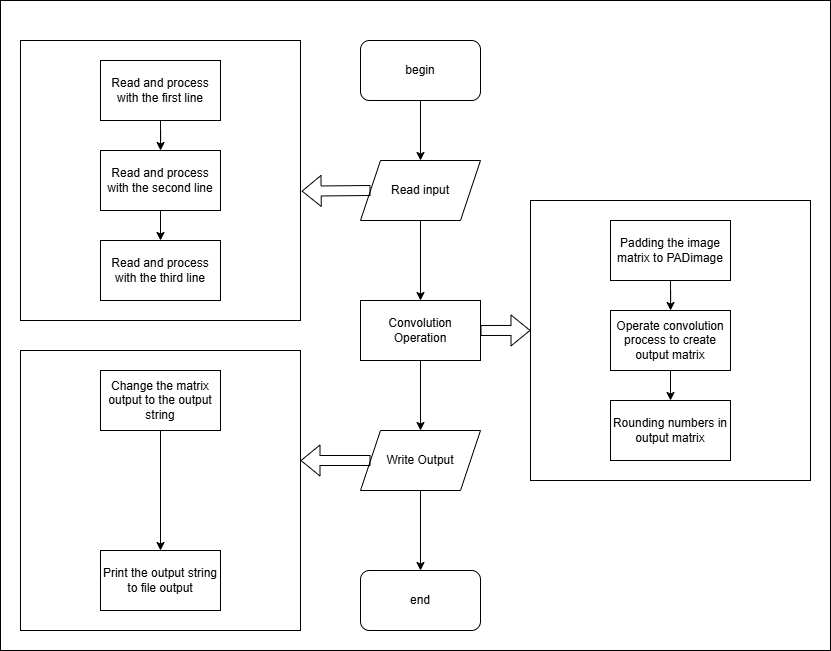
\includegraphics[scale=0.5]{FlowChartForConvolutionOperator.png}
\end{figure}
\pagebreak
\section*{Kiểm thử và đánh giá}
\addcontentsline{toc}{section}{\protect\numberline{}Kiểm thử và đánh giá hiệu suất}
\setcounter{section}{1}\setlength{\baselineskip}{15pt}
% đếm số cho section2, nếu không là hiện 0.1, 0.1.1
\setcounter{subsection}{0}
\setcounter{subsubsection}{0}
\large
\subsection{Kiểm thử}
\subsubsection{Testcase 1}
\begin{lstlisting}[language=,basicstyle=\ttfamily\small]
	Input 1:
	6.0 4.0 3.0 3.0
	2.1 -2.1 2.1 -2.1 2.1 -2.1 2.1 -2.1 2.1 -2.1 2.1 -2.1 1.9 0.1 2.3 -1.1 0.0 8.7 5.3 3.5 1.5 0.9 7.1 -1.2 -1.2 -1.2 -1.2 -2.1 3.4 1.2 2.2 9.9 9.1 0.3 -2.1 1.1
	-3.3 3.4 5.5 6.7 -7.7 6.9 0.0 0.0 7.1 3.3 7.0 0.0 0.0 0.0 0.0 0.0
\end{lstlisting}
\begin{lstlisting}[language=,basicstyle=\ttfamily\small]
	Output 1:
	0.0 0.0 0.0 14.1 -17.3 86.3 35.5 121.6 57.1
\end{lstlisting}
\subsubsection{Testcase 2}
\begin{lstlisting}[language=,basicstyle=\ttfamily\small]
	Input 2:
	3.0 4.0 0.0 3.0
	4.5 5.6 2.3 7.9 -3.4 6.1 -1.9 9.2 4.2
	-3.3 3.4 5.5 6.7 -7.7 6.9 0.0 0.0 7.1 3.3 7.0 0.0 0.0 0.0 0.0 0.0
\end{lstlisting}
\begin{lstlisting}[language=,basicstyle=\ttfamily\small]
	Output 2:
	Error: size not match
\end{lstlisting}
\subsubsection{Testcase 3}
\begin{lstlisting}[language=,basicstyle=\ttfamily\small]
	Input 3:
	4.0 4.0 0.0 3.0
	4.5 5.6 2.3 7.9 -3.4 6.1 -1.9 9.2 4.2 3.5 1.5 0.9 7.1 -1.2 2.2 -1.2
	-3.3 3.4 5.5 6.7 -7.7 6.9 0.0 0.0 7.1 3.3 7.0 0.0 0.0 0.0 0.0 0.0
\end{lstlisting}
\begin{lstlisting}[language=,basicstyle=\ttfamily\small]
	Output 3:
	189.9
\end{lstlisting}
\subsubsection{Testcase 4}
\begin{lstlisting}[language=,basicstyle=\ttfamily\small]
	Input 4:
	5.0 3.0 0.0 1.0
	7.6 -5.5 2.1 0.0 -3.0 4.0 1.0 3.9 1.0 -7.2 9.1 3.2 1.4 5.4 3.2 0.0 3.9 1.0 1.0 3.1 4.6 -1.2 1.6 -1.9 4.0
	1.5 6.0 -12.0 0.0 7.1 0.0 -4.2 6.1 1.3
\end{lstlisting}
\begin{lstlisting}[language=,basicstyle=\ttfamily\small]
	Output 4:
	-56.6 34.2 77.5 13.0 13.9 142.5 19.2 -32.2 -9.9
\end{lstlisting}
\subsubsection{Testcase 5}
\begin{lstlisting}[language=,basicstyle=\ttfamily\small]
	Input 5:
	5.0 3.0 0.0 1.0
	1.2 -1.2 1.2 -1.2 1.2 -1.2 1.2 -1.2 1.2 -1.2 1.2 -1.2 1.2 -1.2 1.2 -1.2 1.2 -1.2 1.2 1.2 -1.2 1.2 -1.2 1.2 -1.2
	-0.0 -0.0 -0.0 -0.0 2.2 3.3 4.4 5.5 6.6
\end{lstlisting}
\begin{lstlisting}[language=,basicstyle=\ttfamily\small]
	Output 5:
	5.3 -5.3 5.3 -5.3 5.3 10.6 -7.9 7.9 0.0
\end{lstlisting}
\subsection{Đánh giá}
\subsubsection{Ưu điểm của MIPS trong phép tích chập}
\begin{itemize}
	\item \textbf{Hiệu suất cao:} MIPS cho phép truy cập phần cứng trực tiếp, tối ưu hiệu suất cho các ứng dụng tính toán thời gian thực.
	\item \textbf{Kiểm soát tài nguyên:} Có thể quản lý tài nguyên phần cứng chi tiết, phù hợp với các hệ thống nhúng.
	\item \textbf{Tối ưu tính toán:} MIPS sử dụng kiến trúc RISC và pipeline, giúp tăng tốc độ xử lý các phép tính.
\end{itemize}
\subsubsection{Nhược điểm của MIPS trong phép tích chập}
\begin{itemize}
	\item \textbf{Mã lệnh dài và khó viết:} Cần nhiều dòng mã để thực hiện một phép toán đơn giản, làm tăng độ phức tạp.
	\item \textbf{Dễ mắc lỗi và khó bảo trì:} Việc viết mã thủ công ở cấp độ thấp khiến dễ xảy ra lỗi và khó kiểm tra, bảo trì.
	\item \textbf{Thiếu thư viện hỗ trợ:} MIPS không có sẵn thư viện cho các phép toán phức tạp như ma trận hay cho việc thao tác và chuyển đổi với chuỗi.
\end{itemize}
\pagebreak


\section*{Kết luận}
\addcontentsline{toc}{section}{\protect\numberline{}Kết luận}
\setcounter{section}{1}\setlength{\baselineskip}{15pt}
% đếm số cho section2, nếu không là hiện 0.1, 0.1.1
\setcounter{subsection}{0}
\setcounter{subsubsection}{0}
\large
\hspace{0.4cm}Phép toán tích chập (convolution) là một thành phần quan trọng trong học sâu, đặc biệt trong mạng nơ-ron tích chập (CNN). Nó giúp mạng học và trích xuất các đặc trưng có giá trị từ dữ liệu hình ảnh, hỗ trợ trong nhiều ứng dụng như nhận diện đối tượng, phân loại ảnh và phân tích video.\medskip

Báo cáo này đã trình bày chi tiết các bước thực hiện phép toán tích chập, từ việc xử lý đầu vào, áp dụng padding, đến việc thực hiện tích chập để tạo ra ma trận đầu ra. Các bước này đều đóng vai trò then chốt trong việc xây dựng đoạn mã.\medskip

Tích chập không chỉ là một phép toán cơ bản mà còn là công cụ mạnh mẽ trong các mô hình học sâu hiện đại, đóng góp vào sự phát triển của các ứng dụng xử lý hình ảnh và video, đồng thời giúp cải thiện khả năng tối ưu hóa và tùy chỉnh mạng nơ-ron.

\end{document}
